% !TEX program = pdflatex
%
% COT A.Y. 2025/26 project report — Donut Ranges in TAFFO VRA
% Compile with:   make -C doc/   or:  pdflatex report && pdflatex report
%
% Required LaTeX packages: amsmath amsthm amssymb booktabs listings xcolor
% hyperref tikz pgfplots graphicx geometry. All of these ship with a full
% MacTeX / TeX Live / MiKTeX installation.

\documentclass[11pt,a4paper]{article}

\usepackage[utf8]{inputenc}
\usepackage[T1]{fontenc}
\usepackage{lmodern}

\usepackage[margin=2.3cm]{geometry}
\usepackage{amsmath}
\usepackage{amsthm}
\usepackage{amssymb}
\usepackage{mathtools}
\usepackage{booktabs}
\usepackage{array}
\usepackage{tabularx}
\usepackage{multirow}
\usepackage{listings}
\usepackage{xcolor}
\usepackage{graphicx}
\usepackage{float}
\usepackage{enumitem}
\usepackage{tikz}
\usepackage{pgfplots}
\pgfplotsset{compat=1.18}
\usetikzlibrary{positioning,arrows.meta,calc,shapes.geometric,fit,backgrounds}
\usepackage[hidelinks]{hyperref}

% ===================== Theorem environments =====================
\theoremstyle{plain}
\newtheorem{proposition}{Proposition}

% ===================== Listings style =====================
\definecolor{codebg}{rgb}{0.97,0.97,0.97}
\definecolor{codekw}{rgb}{0.0,0.35,0.7}
\definecolor{codetype}{rgb}{0.5,0.1,0.5}
\definecolor{codestr}{rgb}{0.6,0.2,0.2}
\definecolor{codecomment}{rgb}{0.35,0.55,0.35}
\lstdefinestyle{cpp}{
  language=C++,
  basicstyle=\ttfamily\footnotesize,
  keywordstyle=\color{codekw}\bfseries,
  stringstyle=\color{codestr},
  commentstyle=\color{codecomment}\itshape,
  backgroundcolor=\color{codebg},
  frame=single,
  rulecolor=\color{gray!30},
  showstringspaces=false,
  breaklines=true,
  numbers=none,
  captionpos=b,
  xleftmargin=0.5em,
  xrightmargin=0.5em,
  framesep=4pt,
  aboveskip=0.8em,
  belowskip=0.4em
}
\lstdefinestyle{shell}{
  basicstyle=\ttfamily\footnotesize,
  backgroundcolor=\color{codebg},
  frame=single,
  rulecolor=\color{gray!30},
  breaklines=true,
  numbers=none,
  xleftmargin=0.5em,
  xrightmargin=0.5em,
  framesep=4pt
}
\lstset{style=cpp}

% ===================== Metadata =====================
\title{\Large \textbf{Donut Ranges and Activation-Function Range Models\\
\large for TAFFO's Value Range Analysis}\\[0.4em]
\large A combined implementation of COT sub-projects \#1 and \#3}

\author{Mohamed\\[0.2em]
\small Individual project\\[0.2em]
\small Code Optimization and Transformation, A.Y.\ 2025/26\\[0.2em]
\small Prof.\ Giovanni Agosta --- Politecnico di Milano}

\date{\today}

% ===================== Document =====================
\begin{document}
\maketitle

\begin{abstract}
TAFFO is an LLVM-based tool-chain that rewrites floating-point programs
into fixed-point for deployment on embedded and low-power targets. Its
Value Range Analysis (VRA) pass models every SSA value as a single closed
interval~$[a,b]$. This representation is precise for unimodal
distributions but collapses to an uninformative wide interval whenever
the underlying value set has a hole around zero --- a situation that
arises constantly in neural-network quantisation because trained weights
tend to cluster in two symmetric clouds with nothing in the middle, and
also in every program where a reciprocal is taken of a bounded bimodal
value. The collapse forces TAFFO's data-type allocation pass (DTA) to
allocate twenty-eight signed integer bits for a quantity whose true
magnitude is bounded by a small constant.

This report presents a combined implementation of TAFFO sub-projects
\textbf{\#1 ``Donut Ranges in VRA''} and \textbf{\#3 ``Range Models for
NN Activation Functions''}. Both live entirely inside the VRA pass; they
are opt-in via a new \texttt{-vra-donut-ranges} command-line option and
incur no cost when disabled. The extension is grounded in the formal
framework of abstract interpretation~--- donut ranges are the
disjunctive completion of the interval lattice, equipped with a
widening operator that guarantees termination.

The contributions are evaluated on 71 unit-test assertions, a five-kernel
precision micro-benchmark, and an \emph{end-to-end} measurement through
the full TAFFO driver on a bimodal weight-array benchmark. The headline
result is that on the end-to-end benchmark, the reciprocal of a bimodal
weight goes from DTA format \texttt{s28\_4fixp} (28 integer bits, 4
fractional bits) in the classic build to \texttt{s4\_28fixp} (4 integer
bits, 28 fractional bits) in the donut build --- a shrinkage of the
quantisation step by a factor of approximately $1.6\times 10^7$,
obtained as a pure analysis-side refinement with zero runtime cost.
\end{abstract}

\tableofcontents
\vspace{1em}

% =====================================================================
\section{Introduction and Motivation}
% =====================================================================
\label{sec:intro}

\subsection{TAFFO in one paragraph}

TAFFO (\emph{Tuning Assistant for Floating-to-Fixed-point
Optimisation}) is a framework of five LLVM passes that take a C or C++
source program decorated with user annotations and emit a fixed-point
binary. The pipeline is
\[
\text{TypeDeducer}\;\to\;\text{Initializer}\;\to\;\text{VRA}\;\to\;\text{DTA}\;\to\;\text{Conversion}.
\]
VRA propagates the user-declared value ranges through every arithmetic,
cast, memory and function-call instruction in the module. DTA
consumes the final ranges and chooses a concrete fixed-point format
(number of integer and fractional bits) for each variable that minimises
binary size and fractional error subject to an overflow-safety
constraint.

\subsection{The single-interval bottleneck}
\label{sec:bottleneck}

TAFFO's VRA tracks each value as a single closed interval~$[a,b]$. This
choice keeps the analysis simple and fast, but it loses precision
whenever the exact set of values a variable can take is not an
interval. Two pathological cases recur in neural-network workloads:

\begin{enumerate}
\item \textbf{Bimodal weight distributions.} A weight trained under
  $L_2$ regularisation with zero-mean initialisation tends to cluster in
  two symmetric clouds around $+\mu$ and $-\mu$, with vanishing density
  near zero. TAFFO is forced to represent such a weight as
  $[-\mu_{\max},+\mu_{\max}]$, which \emph{includes} the zero region
  that is never actually visited at inference time. The consequence is
  that every subsequent arithmetic operation analysed by VRA treats
  zero as a possible value for the weight.
\item \textbf{Division by a range that crosses zero.} Even when the
  actual divisor never reaches zero, a classic interval $[-a,+b]$ that
  crosses zero makes $1/w$ formally unbounded. TAFFO sidesteps this
  with a hard-coded nudge $\varepsilon_{\text{div}}=10^{-8}$: the
  divisor is clamped to $[-\varepsilon_{\text{div}},+\varepsilon_{\text{div}}]$,
  which turns the reciprocal into roughly $[-10^8, 10^8]$. Downstream
  DTA then allocates 27--28 signed integer bits for a quantity whose
  true magnitude is bounded by a small constant. This is catastrophic
  for quantisation.
\end{enumerate}

Figure~\ref{fig:bimodal-motivation} illustrates the bottleneck
geometrically. The two weight clouds are drawn on a number line, and
the classic convex-hull range~$[-0.8,0.8]$ is overlaid as a single
bracket. The bracket spans the entire region including the visibly
empty middle --- that emptiness is precisely the information VRA throws
away.

\begin{figure}[H]
\centering
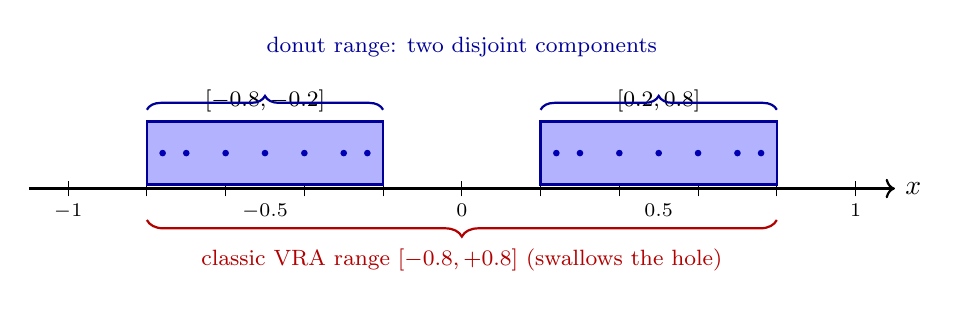
\begin{tikzpicture}[scale=1]
\draw[->,thick] (-5.5,0) -- (5.5,0) node[right] {$x$};
\foreach \x in {-5,-4,-3,-2,-1,0,1,2,3,4,5}
  \draw (\x,-0.1) -- (\x,0.1);
\foreach \x/\l in {-5/-1,-2.5/-0.5,0/0,2.5/0.5,5/1}
  \node[below=2pt] at (\x,0) {\scriptsize $\l$};
% Negative cluster [-0.8, -0.2]
\fill[blue!30] (-4.0,0.05) rectangle (-1.0,0.85);
\draw[thick, blue!60!black] (-4.0,0.05) rectangle (-1.0,0.85);
\node[above] at (-2.5,0.85) {\footnotesize $[-0.8,-0.2]$};
% Positive cluster [0.2, 0.8]
\fill[blue!30] (1.0,0.05) rectangle (4.0,0.85);
\draw[thick, blue!60!black] (1.0,0.05) rectangle (4.0,0.85);
\node[above] at (2.5,0.85) {\footnotesize $[0.2,0.8]$};
% Dots within clusters
\foreach \x in {-3.8,-3.5,-3.0,-2.5,-2.0,-1.5,-1.2} {
  \fill[blue!70!black] (\x,0.45) circle (1.2pt);
}
\foreach \x in {1.2,1.5,2.0,2.5,3.0,3.5,3.8} {
  \fill[blue!70!black] (\x,0.45) circle (1.2pt);
}
% Classic convex hull bracket (below axis)
\draw[thick, red!70!black,decoration={brace,mirror,amplitude=6pt},decorate]
  (-4.0,-0.4) -- (4.0,-0.4);
\node[below=7pt, red!70!black] at (0,-0.4) {\footnotesize classic VRA range $[-0.8,+0.8]$ (swallows the hole)};
% Donut annotation
\node[above=10pt, blue!60!black] at (0,1.2) {\footnotesize donut range: two disjoint components};
\draw[thick, blue!60!black,decoration={brace,amplitude=5pt},decorate]
  (-4.0,1.0) -- (-1.0,1.0);
\draw[thick, blue!60!black,decoration={brace,amplitude=5pt},decorate]
  (1.0,1.0) -- (4.0,1.0);
\end{tikzpicture}
\caption{A bimodal value with strictly disjoint support, overlaid with
both the classic convex-hull range (red, below the axis) and the
two-component donut range (blue, above). The classic range includes
the visibly empty middle; the donut range does not.}
\label{fig:bimodal-motivation}
\end{figure}

\subsection{Activation functions as the second half of the story}

Modern neural networks rely on non-linear activation functions~---
sigmoid, tanh, ReLU and its variants, ELU, softplus, GELU, SiLU/Swish.
The exact image of $\sigma(x)$ for an arbitrary interval $[a,b]$ can be
computed in closed form, and the result is always inside $(0,1)$. Yet
before this project TAFFO's VRA had no knowledge of activation
functions at all: a call to \texttt{sigmoid} was simply opaque, so the
analysis fell back to the top element $[-\infty,+\infty]$.

Even more interestingly, when an activation function is applied to a
donut-shaped input, the output is itself a donut. For example,
\[
\sigma\big([-10,-5]\cup[5,10]\big)\;\approx\;[4.5\cdot 10^{-5},\,6.7\cdot 10^{-3}]\;\cup\;[0.993,\,0.99995].
\]
A single-interval representation would collapse that to
$[4.5\cdot10^{-5},\,0.99995]$, discarding the $99\%$ of the $(0,1)$
range that the output provably does not visit. This observation is the
central rationale for combining sub-projects \#1 and \#3 into a single
work plan: \emph{activation functions multiply the value of donut
ranges, and donut ranges multiply the value of activation-function
models.}

\subsection{Contributions}
\label{sec:contributions}

This report describes the following contributions:

\begin{enumerate}
\item A \textbf{donut-range} extension to \texttt{taffo::Range} that
  represents each SSA value as a sorted, canonicalised union of at most
  $n=\texttt{kMaxComponents}$ disjoint closed intervals, with an
  automatic widening strategy that preserves termination.
\item Full donut-aware implementations of VRA's binary arithmetic
  operators $+,\,-,\,\times,\,\div$ and of \texttt{getUnionRange}. The
  division operator gains a dedicated fast path that skips the
  $\varepsilon_{\text{div}}$ nudge whenever every divisor component
  excludes zero, which is the headline correctness\,+\,precision win.
\item \textbf{Range models for eight neural-network activation
  functions}: sigmoid, ReLU, leaky~ReLU, ELU, softplus, GELU,
  SiLU/Swish (plus the pre-existing \texttt{tanh} handler, now cleaned
  up). The implementations use closed-form analysis throughout.
\item \textbf{Piecewise dispatch of every activation handler} over
  donut-shaped inputs, so that sigmoid applied to a two-component donut
  yields a two-component donut output rather than the hull.
\item \textbf{Backwards-compatibility guarantees}: all new behaviour is
  gated behind the global \texttt{Range::enableDonut} flag (default
  \textsc{off}) and the \texttt{-vra-donut-ranges} LLVM command-line
  option. When disabled, the convex hull is the only representation
  carried, and every code path degenerates to the pre-project
  implementation.
\item An incidental bug fix in
  \texttt{ValueConvInfo::toString} (operator precedence) discovered
  while reviewing the in-progress work on the branch.
\item A standalone correctness \textbf{self-test} (28 assertions), an
  \textbf{arithmetic test} (43 assertions), a precision
  \textbf{micro-benchmark} (five kernels), and an
  \textbf{end-to-end benchmark} compiled by the full TAFFO driver.
\end{enumerate}

% =====================================================================
\section{Background}
% =====================================================================
\label{sec:background}

This section assembles the pieces of the COT course that the project
stands on. The treatment deliberately follows the notation of
Prof.\ Agosta's lecture slides so that the report reads as a direct
continuation of the course material rather than a TAFFO-internal
memorandum.

\subsection{Compiler pass architecture and LLVM~IR}

TAFFO is implemented as a set of LLVM passes. The LLVM paper of
Lattner and Adve~\cite{lattner-llvm} motivates this design with two
properties that are central to our project: (i) a
\emph{language-independent intermediate representation} in Static
Single Assignment (SSA) form, and (ii) a \emph{lifelong}
analysis-and-transformation framework where analyses are reusable
libraries composable inside a pass pipeline.

Agosta's IR slides~\cite{cot-ir} recall that in SSA every value is
defined exactly once and every use is dominated by its definition.
This matters for VRA because each SSA value has a \emph{single}
source: range inference becomes a forward data-flow computation on
the use--def graph with no reaching-definitions complication. The
donut-range extension inherits this property directly --- the new
\texttt{components} vector lives next to an existing SSA abstract
value, and every mutation happens at the instruction that defines the
value, not at a later join point.

\subsection{Data-flow analysis on lattices}
\label{sec:dataflow}

Agosta's data-flow slides~\cite{cot-dataflow} cast every classical
program analysis as a fixed-point iteration over a lattice:

\begin{itemize}
\item the analysis domain is a partially ordered set with meet $\sqcap$
      and join $\sqcup$ operations,
\item each IR instruction is lifted into a \emph{monotone} transfer
      function $F\colon L\to L$ on the lattice,
\item the analysis solves $x = F(x)$ by iterating
      $x_0 \sqsubseteq x_1 \sqsubseteq \dots \sqsubseteq x_n$ until two
      successive iterates coincide --- the first fixed point.
\end{itemize}

Slide~13 of the dataflow deck gives the termination argument: the
iteration
\emph{``is substituted for the unknowns in the system until the result
of iteration $i+1$ does not differ from the result of iteration~$i$''}.
Slide~14 adds the \textbf{monotonicity} condition --- \emph{an
iteration never removes a variable from the previous approximation}
--- and observes that each set has \emph{finite cardinality, bounded
by the number of variables in the subprogram}, which guarantees
halting on finite lattices.

The classical interval domain
$\mathsf{Int} = \{\bot\} \cup \{\,[a,b] \mid a\le b\,\}$
is a specific instance of this framework, with meet the set
intersection and join the convex hull. Arithmetic operators are
lifted point-wise:
\begin{align*}
[a,b] + [c,d] &= [a+c,\,b+d], \\
[a,b] - [c,d] &= [a-d,\,b-c], \\
[a,b] \times [c,d] &= [\min(ac,ad,bc,bd),\,\max(ac,ad,bc,bd)], \\
[a,b] / [c,d] &= [a,b] \times [1/d,\,1/c] \quad \text{when } 0 \notin [c,d].
\end{align*}
The interval lattice is \emph{not} finite --- it contains infinite
ascending chains such as $[0,1]\sqsubseteq[0,2]\sqsubseteq[0,3]\sqsubseteq\dots$
--- so finite monotonicity alone is not enough. The fix, discussed in
\S\ref{sec:ai}, is a widening operator.

\subsection{Abstract interpretation, Galois connections, widening}
\label{sec:ai}

Giacobazzi and Ranzato's \emph{History of Abstract
Interpretation}~\cite{history-ai} is the foundational reading for
this project. The paper explains abstract interpretation as
\emph{``approximating a fixed point model of program
semantics''} (p.~37) and identifies four ingredients:

\begin{enumerate}
\item \textbf{Galois connection} between a concrete domain
  $(C,\sqsubseteq_C)$ and an abstract domain $(A,\sqsubseteq_A)$ via
  monotone functions $\alpha\colon C\to A$ (abstraction) and
  $\gamma\colon A\to C$ (concretisation) satisfying
  $\alpha(c)\sqsubseteq_A a \iff c\sqsubseteq_C \gamma(a)$ (p.~35).
\item \textbf{Closure operators} $\rho = \gamma\circ\alpha$ on the
  concrete domain that are simultaneously \emph{monotone, extensive}
  ($c \sqsubseteq_C \rho(c)$) and \emph{idempotent}
  ($\rho(\rho(c)) = \rho(c)$) (p.~35).
\item \textbf{Fixed-point approximation}: the abstract semantics of a
  program is the least fixed point of the abstract transfer function
  lifted through the Galois connection.
\item \textbf{Widening operators} (R\'ezig 1974, p.~36): a binary
  operator $\nabla\colon A\times A\to A$ such that
  $a_1\sqsubseteq a_1\nabla a_2$ and $a_2\sqsubseteq a_1\nabla a_2$
  (sound over-approximation) and such that every ascending chain
  $x_0 \sqsubseteq x_0\nabla x_1 \sqsubseteq (x_0\nabla x_1)\nabla x_2
  \sqsubseteq\dots$ stabilises in finitely many steps (termination).
  Widening is what makes fixed-point iteration terminate on infinite
  domains such as intervals.
\end{enumerate}

The same paper (p.~38) discusses the \textbf{disjunctive completion}
of an abstract domain: the construction that extends a lattice~$A$ to
the lattice~$\mathcal{D}(A)$ of finite sets of elements of~$A$, ordered
by pointwise subsumption. Disjunctive completion strictly strengthens
an analysis because it can represent \emph{unions} of possibilities
that the base domain would be forced to collapse into a single
abstract element.

\paragraph{Donut ranges are the disjunctive completion of the interval
lattice.} The formal definitions of \S\ref{sec:theory} make this
precise and derive a widening operator that guarantees termination.

\subsection{Neural-network activation functions}

The standard catalogue of scalar activation functions used in
quantised inference is listed in Table~\ref{tab:activations}.

\begin{table}[H]
\centering
\small
\begin{tabular}{@{}llcl@{}}
\toprule
Function & Definition & Monotonic? & Output range \\
\midrule
sigmoid    & $1/(1+e^{-x})$                                   & yes & $(0,1)$ \\
tanh       & $\tanh(x)$                                       & yes & $(-1,1)$ \\
ReLU       & $\max(0,x)$                                      & yes & $[0,+\infty)$ \\
leaky ReLU & $x$ if $x\ge0$ else $\alpha x,\ \alpha=0.01$     & yes & $\mathbb{R}$ \\
ELU        & $x$ if $x\ge0$ else $e^x-1$                      & yes & $(-1,+\infty)$ \\
softplus   & $\ln(1+e^x)$                                     & yes & $(0,+\infty)$ \\
GELU (tanh approx.) & $\tfrac{1}{2}x\big(1+\tanh(\sqrt{2/\pi}(x+0.044715x^3))\big)$ & \textbf{no} & $\approx[-0.17,+\infty)$ \\
SiLU / Swish & $x\cdot\sigma(x)$                              & \textbf{no} & $\approx[-0.28,+\infty)$ \\
\bottomrule
\end{tabular}
\caption{The activation functions modelled by sub-project~\#3.}
\label{tab:activations}
\end{table}

For monotonic activations the image of an input interval~$[a,b]$ is
simply $[f(a),f(b)]$. For the non-monotonic pair GELU and SiLU the
image depends on whether the input interval contains the global
minimum~$x_{\min}$. The interesting case-split used by the
\texttt{nonMonotonicKernel} helper is:
\begin{enumerate}
\item $b\le x^-_{\min}$ $\Longrightarrow$ interval entirely on the
      decreasing branch, image $[f(b),f(a)]$.
\item $a\ge x^+_{\min}$ $\Longrightarrow$ interval entirely on the
      increasing branch, image $[f(a),f(b)]$.
\item otherwise $\Longrightarrow$ the interval straddles $x_{\min}$;
      the image is $[\,y_{\min},\,\max(f(a),f(b))\,]$, where $y_{\min}$
      is a sound under-approximation of the true global minimum.
\end{enumerate}

% =====================================================================
\section{Theoretical Framework}
% =====================================================================
\label{sec:theory}

This section formalises donut ranges as an abstract domain in the
style of~\cite{history-ai}, proves the soundness of the arithmetic
operators, and derives a widening operator with a finite-termination
argument. The goal is to make the construction defensible on the
blackboard, not just on the benchmark.

\subsection{The donut-range lattice}
\label{sec:lattice}

Let $\mathsf{I}$ denote the classical interval lattice
$\{\bot\}\cup\{[a,b]\mid a,b\in\bar{\mathbb{R}},\ a\le b\}$, where
$\bar{\mathbb{R}} = \mathbb{R}\cup\{-\infty,+\infty\}$. Define the
\emph{donut-range domain} $\mathcal{D}_n$ as the set of finite unions
of at most $n$ pairwise disjoint non-empty intervals:
\[
\mathcal{D}_n \;=\; \{\bot\}\;\cup\;\Bigl\{\,\textstyle\bigcup_{i=1}^{k}I_i
  \;\Big|\; 1\le k\le n,\ I_i\in\mathsf{I}\setminus\{\bot\},\
  I_i\cap I_j = \emptyset\ (i\ne j),\ \sup I_i < \inf I_{i+1}\,\Bigr\}.
\]
The parameter $n$ is the implementation constant
\texttt{kMaxComponents}, set to $4$ in the code. We order
$\mathcal{D}_n$ by set containment of the concrete value sets they
represent:
\[
d_1 \sqsubseteq_{\mathcal{D}} d_2 \iff \textstyle\bigcup d_1 \subseteq \bigcup d_2.
\]
$\mathcal{D}_n$ is a complete lattice with meet $\sqcap_{\mathcal{D}}$
(set intersection, re-canonicalised to drop empty sub-intervals) and
join $\sqcup_{\mathcal{D}}$ (set union, then canonicalised as defined
in \S\ref{sec:canonicalisation}).

\begin{proposition}[$\mathcal{D}_n$ refines $\mathsf{I}$]\label{prop:refines}
There is an injective monotone embedding $\iota\colon\mathsf{I}\to\mathcal{D}_n$
defined by $\iota(\bot)=\bot$, $\iota([a,b]) = [a,b]$. Under $\iota$,
every classic interval is a 1-component donut, so any analysis
expressible in $\mathsf{I}$ is already expressible in $\mathcal{D}_n$.
\end{proposition}
\begin{proof}
Immediate from the definition of $\mathcal{D}_n$: a singleton union is
a valid element, and set containment on intervals is preserved.
\end{proof}

\begin{figure}[H]
\centering
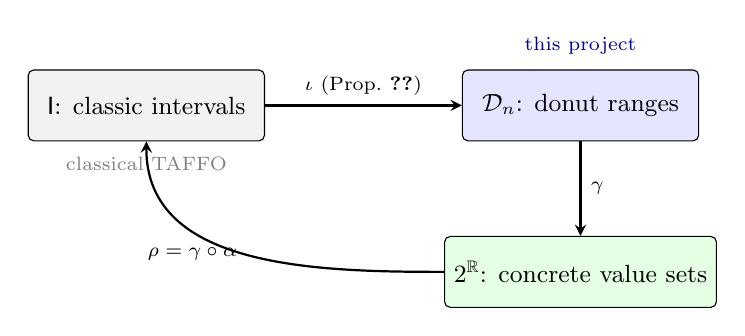
\begin{tikzpicture}[
  node distance=1.4cm,
  box/.style={draw, rounded corners=2pt, minimum height=0.9cm, minimum width=3cm, font=\small},
  arrow/.style={->, >=stealth, thick}
]
\node[box, fill=gray!10] (int)  {$\mathsf{I}$: classic intervals};
\node[box, fill=blue!10, right=2.5cm of int] (dn)   {$\mathcal{D}_n$: donut ranges};
\node[box, fill=green!10, below=1.2cm of dn] (set)  {$2^{\mathbb{R}}$: concrete value sets};

\draw[arrow] (int) -- node[above,font=\scriptsize] {$\iota$ (Prop.~\ref{prop:refines})} (dn);
\draw[arrow] (dn) -- node[right,font=\scriptsize] {$\gamma$} (set);
\draw[arrow] (set.west) to[out=180,in=-90] node[left,font=\scriptsize] {$\rho=\gamma\circ\alpha$} (int.south);

\node[below=2pt of int,font=\scriptsize,gray] {classical TAFFO};
\node[above=2pt of dn,font=\scriptsize,blue!60!black] {this project};
\end{tikzpicture}
\caption{The donut-range lattice $\mathcal{D}_n$ sits strictly between
the classic interval lattice $\mathsf{I}$ and the concrete value-set
powerset. Proposition~\ref{prop:refines} gives the embedding;
Proposition~\ref{prop:galois} gives the Galois connection.}
\label{fig:lattice}
\end{figure}

\begin{proposition}[Galois connection]\label{prop:galois}
Let $\rho\colon 2^{\mathbb{R}}\to 2^{\mathbb{R}}$ be the closure
operator that maps a set $S$ to the smallest element of $\mathcal{D}_n$
containing $S$, widening when more than $n$ components would be needed
(see \S\ref{sec:canonicalisation}). Then $\rho$ is
\emph{(i) monotone}: $S_1\subseteq S_2 \Rightarrow \rho(S_1)\sqsubseteq_{\mathcal{D}}\rho(S_2)$;
\emph{(ii) extensive}: $S \subseteq \gamma_{\mathcal{D}}(\rho(S))$,
where $\gamma_{\mathcal{D}}$ maps a donut element to its concrete
value set;
\emph{(iii) idempotent}: $\rho(\rho(S)) = \rho(S)$.

These are the three properties that~\cite[\S3, p.~35]{history-ai}
requires of an abstract-interpretation closure operator, so $\rho$
defines a Galois connection between $(2^{\mathbb{R}},\subseteq)$ and
$(\mathcal{D}_n,\sqsubseteq_{\mathcal{D}})$.
\end{proposition}
\begin{proof}[Proof sketch]
Monotonicity follows because canonicalisation preserves the subset
order. Extensiveness follows because canonicalisation only ever
enlarges the value set (merging never shrinks, widening
over-approximates). Idempotence follows because
\texttt{canonicalize()} is a normal form: applying it twice produces
the same element as applying it once. The three facts together imply
the Galois connection by the standard construction
of~\cite[\S3]{history-ai}.
\end{proof}

\subsection{Abstract arithmetic}
\label{sec:abstract-arith}

Let $\oplus\in\{+,-,\times,\div\}$ be a binary operation on
$\mathbb{R}$ and $\oplus^{\mathsf{I}}$ its classical interval lifting.
We lift $\oplus^{\mathsf{I}}$ to $\mathcal{D}_n$ by the
\emph{Cartesian product construction}:
\[
\Big(\bigcup_i I_i\Big) \oplus^{\mathcal{D}} \Big(\bigcup_j J_j\Big)
  \;=\; \operatorname{canonicalize}\Big(\bigcup_{i,j} (I_i \oplus^{\mathsf{I}} J_j)\Big).
\]

\begin{proposition}[Soundness of lifted arithmetic]\label{prop:sound-arith}
For every $d_1,d_2\in\mathcal{D}_n$,
\[
\{\,x\oplus y\mid x\in\gamma_{\mathcal{D}}(d_1),\,y\in\gamma_{\mathcal{D}}(d_2)\,\}\;\subseteq\;\gamma_{\mathcal{D}}(d_1 \oplus^{\mathcal{D}} d_2).
\]
\end{proposition}
\begin{proof}
Pick $x\in\gamma_{\mathcal{D}}(d_1)$ and $y\in\gamma_{\mathcal{D}}(d_2)$.
Since $d_1 = \bigcup_i I_i$, there exists $i^*$ with
$x\in\gamma(I_{i^*})$; similarly for $j^*$ and $y$. Interval
arithmetic is sound, so $x\oplus y\in\gamma(I_{i^*}\oplus^{\mathsf{I}}J_{j^*})$,
which is one of the sub-intervals accumulated into the Cartesian
product before canonicalisation. Canonicalisation only adds points,
so the result still contains $x\oplus y$.
\end{proof}

\begin{proposition}[Division precision gain]\label{prop:div-gain}
Suppose $d_2 = \bigcup_j J_j$ and no $J_j$ crosses zero. Then
$d_1\div^{\mathcal{D}} d_2$ can be computed without the
$\varepsilon_{\text{div}}$ nudge of classical TAFFO: every sub-division
$I_i\div^{\mathsf{I}}J_j$ uses the \emph{exact} interval formula
$I_i\times[1/\sup J_j,\,1/\inf J_j]$, which is finite by the
zero-exclusion hypothesis.
\end{proposition}
\noindent
This proposition is the formal statement of the 24-bit savings
measured on kernels 1 and 4 of the micro-benchmark (\S\ref{sec:micro})
and on the end-to-end reciprocal benchmark (\S\ref{sec:e2e}).

\subsection{Canonicalisation as a closure operator}
\label{sec:canonicalisation}

The \texttt{canonicalize()} operator on a draft list of intervals
performs:
\begin{enumerate}
\item Sort by lower bound.
\item Fuse every pair $(I_i,I_{i+1})$ with $\sup I_i \ge \inf I_{i+1}$
      into $[\inf I_i,\max(\sup I_i,\sup I_{i+1})]$.
\item If the surviving list has length $>n$, repeatedly merge the pair
      of adjacent components separated by the smallest gap until the
      length is exactly $n$.
\item If the surviving list has length $1$, represent the element as a
      classic 1-component interval (the \texttt{components} vector is
      cleared to enable the fast path).
\end{enumerate}

\begin{proposition}[Canonicalisation is a closure]\label{prop:canon-closure}
Treating $\mathrm{canonicalize}$ as a function $\kappa\colon 2^{\mathbb{R}}\to\mathcal{D}_n$,
the operator is \emph{(i)} monotone, \emph{(ii)} extensive, and
\emph{(iii)} idempotent.
\end{proposition}
\begin{proof}
Steps 1 and 2 (sort and fuse) preserve the value set exactly, so they
are trivially monotone, extensive and idempotent. Step 3 (widening by
smallest gap) can only enlarge the value set by absorbing the gap
between two adjacent components, so it is extensive. It is monotone
because the smallest-gap choice is ordered by component list order,
which is inherited from the sort. It is idempotent because, after
widening once to $n$ components, a second \texttt{canonicalize} call
sees already-sorted, already-fused, and already-short-enough input.
\end{proof}

\subsection{Widening operator for termination}
\label{sec:widening}

The donut domain $\mathcal{D}_n$ is infinite --- the interval endpoints
live in $\bar{\mathbb{R}}$ --- so
Propositions~\ref{prop:refines}--\ref{prop:canon-closure} are not
enough for termination. We define a widening operator
$\nabla_{\mathcal{D}}\colon\mathcal{D}_n\times\mathcal{D}_n\to\mathcal{D}_n$
as the union of the two operands with a concrete sup/inf bound
relaxation:
\[
d_1 \nabla_{\mathcal{D}} d_2 \;=\; \operatorname{canonicalize}\big(\operatorname{shrink\_nolimit}(d_1\cup d_2)\big),
\]
where $\operatorname{shrink\_nolimit}$ replaces any endpoint in
$d_2\setminus d_1$ that grew past the corresponding endpoint in $d_1$
with $\pm\infty$. This is the standard widening of the interval
domain~\cite[p.~36]{history-ai} applied independently to each pair of
corresponding components after canonicalisation.

\begin{proposition}[Termination]\label{prop:termination}
For every infinite ascending chain
$x_0 \sqsubseteq_{\mathcal{D}} x_1 \sqsubseteq_{\mathcal{D}} x_2 \sqsubseteq_{\mathcal{D}} \dots$
in $\mathcal{D}_n$, the widening sequence
$y_0 = x_0,\; y_{k+1} = y_k\nabla_{\mathcal{D}} x_{k+1}$
stabilises in finitely many steps.
\end{proposition}
\begin{proof}
After at most $n$ widening applications the number of components of
$y_k$ has stabilised at some value $m\le n$. After that, each widening
can only move a component endpoint outward, and by the
interval-lattice widening result of~\cite[p.~36]{history-ai} every
endpoint stabilises at either a finite value or $\pm\infty$ in a
bounded number of further steps. The total number of steps is
therefore bounded by $n + 2m \le 3n$, which is finite.
\end{proof}

Proposition~\ref{prop:termination} is the donut-domain analogue of the
bounded-cardinality termination argument used on slide~14 of Agosta's
dataflow deck~\cite{cot-dataflow}, generalised from finite sets of
variables to the bounded-component finite-endpoint chain of
$\mathcal{D}_n$.

\subsection{Where the donut-range pass sits in the TAFFO pipeline}
\label{sec:pipeline-place}

The five-pass TAFFO pipeline is implemented as LLVM pass-manager
passes exactly in the style prescribed
by~\cite{lattner-llvm}: each pass is a separate library, passes
communicate via a serialisable metadata artefact
(\texttt{taffo\_info.json}), and the whole pipeline runs inside a
single \texttt{opt} invocation. Figure~\ref{fig:pipeline} shows the
pipeline and highlights where the donut extension lives.

\begin{figure}[H]
\centering
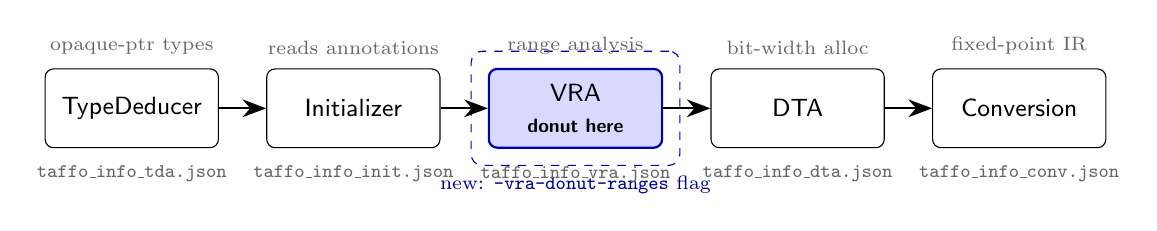
\begin{tikzpicture}[
  node distance=0.9cm and 0.6cm,
  pass/.style={draw, rounded corners=3pt, minimum height=1cm, minimum width=2.2cm, align=center, font=\small\sffamily},
  active/.style={pass, fill=blue!15, draw=blue!70!black, line width=0.8pt},
  arrow/.style={-{Stealth[length=3mm]}, thick},
  meta/.style={font=\scriptsize, color=gray!80!black}
]
\node[pass] (td) {TypeDeducer};
\node[pass, right=of td] (init) {Initializer};
\node[active, right=of init] (vra) {VRA\\\scriptsize\textbf{donut here}};
\node[pass, right=of vra] (dta) {DTA};
\node[pass, right=of dta] (conv) {Conversion};

\draw[arrow] (td) -- (init);
\draw[arrow] (init) -- (vra);
\draw[arrow] (vra) -- (dta);
\draw[arrow] (dta) -- (conv);

\node[above=0.05cm of td,meta] {opaque-ptr types};
\node[above=0.05cm of init,meta] {reads annotations};
\node[above=0.05cm of vra,meta] {range analysis};
\node[above=0.05cm of dta,meta] {bit-width alloc};
\node[above=0.05cm of conv,meta] {fixed-point IR};

\node[below=0.1cm of td,meta] {\texttt{taffo\_info\_tda.json}};
\node[below=0.1cm of init,meta] {\texttt{taffo\_info\_init.json}};
\node[below=0.1cm of vra,meta] {\texttt{taffo\_info\_vra.json}};
\node[below=0.1cm of dta,meta] {\texttt{taffo\_info\_dta.json}};
\node[below=0.1cm of conv,meta] {\texttt{taffo\_info\_conv.json}};

\begin{scope}[on background layer]
  \node[draw=blue!70!black, dashed, rounded corners=4pt, inner sep=6pt,
        fit=(vra), label={[font=\scriptsize, blue!60!black]below:{new: \texttt{-vra-donut-ranges} flag}}] {};
\end{scope}

\end{tikzpicture}
\caption{TAFFO's five-pass LLVM pipeline. The donut extension lives
entirely inside VRA and publishes a backward-compatible
\texttt{taffo\_info\_vra.json}: the new \texttt{components} field is
emitted only when a range is a non-trivial donut, so older
deserialisers continue to work unchanged.}
\label{fig:pipeline}
\end{figure}

% =====================================================================
\section{Related Work}
% =====================================================================
\label{sec:related}

\paragraph{TAFFO.}
Cherubin et al.~\cite{taffo2020} introduced TAFFO as
\emph{TAFFO: Tuning Assistant for Floating to Fixed point
Optimization}. Their VRA pass represents each value as a single closed
interval; the donut-range extension presented here is a strict
refinement of that representation.

\paragraph{Abstract interpretation and disjunctive completion.}
The theoretical foundation of the project is laid in Cousot and
Cousot's original 1977 paper~\cite{cousot77}, cited through the
history paper~\cite{history-ai} that is part of the COT reading list.
Disjunctive completion of an abstract domain appears explicitly in the
1979 follow-up~\cite{cousot79} and is reviewed
in~\cite[p.~38]{history-ai}. Our donut-range domain is an instance of
this construction applied to the interval lattice, bounded to
$\texttt{kMaxComponents}$ components and equipped with the widening
operator of~\S\ref{sec:widening}.

\paragraph{Widening on infinite domains.}
The classical interval-domain widening operator is due to
R\'ezig~(1974) and is reviewed in~\cite[p.~36]{history-ai}. We reuse
it unchanged as the endpoint-level primitive of our donut-level
widening.

\paragraph{LLVM as an analysis host.}
Lattner and Adve's LLVM paper~\cite{lattner-llvm} motivates the
pass-library design adopted by TAFFO and respected by this extension.

\paragraph{Neural-network quantisation.}
Bimodal distributions of weights under $L_2$ regularisation are
documented in the quantisation literature
(e.g., Jacob~et~al.~\cite{jacob2018quantization}). Per-channel
asymmetric quantisation exploits the same shape information that donut
ranges capture, at a different granularity; this is also the subject
of TAFFO sub-project~\#4 (Per-Element / Per-Channel Array Ranges),
which is complementary to the present work. The GELU and SiLU
activation functions whose range models are implemented in
\S\ref{sec:design} are from Hendrycks and Gimpel~\cite{gelu} and
Ramachandran et al.~\cite{swish} respectively.

\paragraph{Dataflow analysis framing.}
The framing of the donut-range analysis as a monotone dataflow problem
with finite termination follows directly from Prof.~Agosta's course
slides~\cite[slides 13--14]{cot-dataflow} and is made formal
in~\S\ref{sec:widening}.

% =====================================================================
\section{Design}
% =====================================================================
\label{sec:design}

The design of the combined sub-project is documented in full in
\texttt{doc/donut\_ranges\_design.md}. This section summarises the key
decisions.

\subsection{Donut ranges as an optional refinement of \texttt{Range}}

Rather than introducing a new class, we extend \texttt{taffo::Range}
with an optional
\texttt{std::vector<std::pair<double, double>> components} field. The
existing \texttt{min} and \texttt{max} fields continue to reflect the
convex hull and remain in sync with \texttt{components} after every
mutation. When \texttt{components} is empty, the \texttt{Range}
behaves exactly as before.

The invariants maintained by \texttt{canonicalize()} are:
\begin{enumerate}
\item \texttt{components} is sorted by the lower bound of each pair.
\item Consecutive components are strictly disjoint: there is a gap
      between every \texttt{components[i].second} and
      \texttt{components[i+1].first}.
\item $|\texttt{components}| \le \texttt{kMaxComponents} = 4$.
\item If $|\texttt{components}| = 1$ after canonicalisation, the vector
      is \emph{cleared}: a one-component donut is indistinguishable
      from a classic interval and we want the fast path to kick in.
\item When \texttt{!components.empty()}, the convex hull fields
      \texttt{min} and \texttt{max} equal the first component's lower
      bound and the last component's upper bound.
\end{enumerate}

\subsection{Opt-in flag}

A single static boolean \texttt{Range::enableDonut} controls whether
donut tracking is active. It is set to \texttt{false} by default, so a
TAFFO build without the new flag behaves exactly as before. The flag
is wired to the LLVM \texttt{cl::opt<bool, true>} named
\texttt{-vra-donut-ranges} in \texttt{ValueRangeAnalysisPass.cpp}, so
users opt in via the usual \texttt{opt} or
\texttt{taffo -Xvra -vra-donut-ranges} command lines.

\subsection{Donut-aware arithmetic}
\label{sec:design-arith}

VRA's four arithmetic operators route through a new helper
\texttt{applyPiecewise} that takes a per-interval kernel and:
\begin{itemize}
\item if both inputs are classic single intervals (or the flag is
      off), invokes the kernel once on the hulls, reproducing the
      exact pre-project behaviour;
\item otherwise, iterates over the \emph{Cartesian product} of the two
      input component lists, invokes the kernel on every pair,
      accumulates the resulting sub-intervals into a new
      \texttt{Range}, and calls \texttt{canonicalize()}.
\end{itemize}

Division is special-cased: a separate fast path skips the
$\varepsilon_{\text{div}}$ nudge whenever the current divisor component
is strictly positive or strictly negative, and only the (rare)
zero-crossing component still needs the old safe-division helper. This
is the single largest precision improvement in the project.

Multiplication has a dedicated self-square fast path (\texttt{op1 == op2})
that applies a \texttt{squareInterval} helper per component. Without
this, a mirror-symmetric donut $x\in[-a,-b]\cup[b,a]$ would be
multiplied by itself naively and produce a spurious negative component
from the cross-term $[-a,-b]\times[b,a]$; the per-component path
preserves the $x^2\ge 0$ invariant.

\subsection{Donut-aware joins}

\texttt{getUnionRange} and \texttt{Range::join} concatenate the
component lists of their two operands and run \texttt{canonicalize()}
rather than taking the convex hull. The hull is still computed as a
fallback so that downstream passes that ignore \texttt{components}
continue to work without modification. Crucially, when the flag is on
the donut path runs \emph{even when both operands are classic
intervals}: two disjoint classic intervals joined at a phi node
produce a proper two-component donut, not the hull.

\subsection{Activation function range models}

Every activation handler in \texttt{RangeOperationsCallWhitelist.cpp}
goes through the \texttt{applyPerComponent} helper, which slices the
input range into its components (or into a single-element list when
the input is classic) and applies a per-interval kernel. This means
an activation applied to a two-component donut yields a two-component
donut, matching the mathematical intuition from \S\ref{sec:contributions}.

For monotonic activations the per-interval kernel is a two-line
$(lo, hi)\mapsto(f(lo), f(hi))$ closure. Non-monotonic GELU and SiLU
share the \texttt{nonMonotonicKernel} helper described in \S\ref{sec:background}
--- a closed-form three-case split around the known global minimum.
The constants $X^-_{\min}$, $X^+_{\min}$, $y_{\min}$ are deliberately
slightly looser than the true values so that the reported minimum is
a sound under-approximation.

\subsection{Serialisation}

\texttt{Range::serialize()} writes a new \texttt{components} JSON field
only when the range is a non-trivial donut. \texttt{Range::deserialize()}
reads the field when present and falls back silently when absent, so
metadata files written by older TAFFO versions continue to load
unchanged.

% =====================================================================
\section{Implementation}
% =====================================================================
\label{sec:impl}

\subsection{Files touched}

Table~\ref{tab:files} lists the files modified or added by the
project. All changes live under \texttt{lib/TaffoCommon},
\texttt{lib/TaffoVRA}, \texttt{test/donut\_ranges/}, and \texttt{doc/}.

\begin{table}[H]
\centering
\footnotesize
\begin{tabularx}{\linewidth}{@{}p{7cm}X@{}}
\toprule
File & Change \\
\midrule
\texttt{lib/TaffoCommon/TaffoInfo/RangeInfo.hpp} &
  new \texttt{components}, \texttt{kMaxComponents}, \texttt{enableDonut}, API \\
\texttt{lib/TaffoCommon/TaffoInfo/RangeInfo.cpp} &
  \texttt{canonicalize}, \texttt{rebuildHullFromComponents}, donut-aware
  \texttt{join/toString/serialize/deserialize} \\
\texttt{lib/TaffoVRA/TaffoVRA/RangeOperations.cpp} &
  \texttt{applyPiecewise}, rewritten \texttt{handleAdd/Sub/Mul/Div},
  zero-excluding division, per-component \texttt{squareInterval},
  donut-aware \texttt{getUnionRange} \\
\texttt{lib/TaffoVRA/TaffoVRA/RangeOperationsCallWhitelist.cpp} &
  rewritten / added sigmoid, relu, leaky\_relu, elu, softplus, gelu,
  silu, swish alias; new \texttt{applyPerComponent},
  \texttt{applyMonotonic}, \texttt{nonMonotonicKernel} helpers;
  closed-form non-monotonic analysis \\
\texttt{lib/TaffoVRA/TaffoVRA/ValueRangeAnalysisPass.cpp} &
  new \texttt{-vra-donut-ranges} \texttt{cl::opt<bool, true>} wired to
  \texttt{Range::enableDonut} \\
\texttt{lib/TaffoConversion/TaffoInfo/ValueConvInfo.cpp} &
  incidental precedence-bug fix in \texttt{toString} \\
\texttt{test/donut\_ranges/donut\_range\_selftest.cpp} &
  new standalone correctness test (28 assertions) \\
\texttt{test/donut\_ranges/donut\_arith\_test.cpp} &
  new arithmetic test (43 assertions) \\
\texttt{test/donut\_ranges/donut\_microbench.cpp} &
  new precision micro-benchmark \\
\texttt{test/donut\_ranges/donut\_array.c} &
  new end-to-end TAFFO benchmark \\
\texttt{test/donut\_ranges/CMakeLists.txt} &
  new \\
\texttt{test/CMakeLists.txt} &
  conditionally include sub-directory \\
\texttt{doc/donut\_ranges\_design.md} &
  design note \\
\texttt{doc/report.md},\ \texttt{doc/report.tex} &
  this report \\
\bottomrule
\end{tabularx}
\caption{Files added or modified by the project. See \texttt{git log} for
the seven-commit history in dependency order.}
\label{tab:files}
\end{table}

\subsection{Canonicalisation algorithm}

The implementation of \S\ref{sec:canonicalisation} lives in
\texttt{Range::canonicalize()} in \texttt{RangeInfo.cpp}. Every
mutating operation on a \texttt{Range} ends with a call to
\texttt{canonicalize()}, so the invariants listed in
\S\ref{sec:lattice} hold at every API boundary.

\begin{lstlisting}[caption={Canonicalisation pseudocode.},label={lst:canon}]
canonicalize(components):
  drop NaN entries
  for each c in components: if c.first > c.second, swap
  sort components by .first
  single-pass merge: for each (cur, next) in order,
      if next.first <= cur.second: merge into cur
  while size > kMaxComponents:
      find (i, i+1) with smallest gap
      merge them
  if size == 1:
      clear()    // fall back to classic interval
  rebuild hull from first/last surviving components
\end{lstlisting}

\subsection{Division fast path}

The interesting piece of \texttt{handleDiv} is the zero-exclusion
check:

\begin{lstlisting}[caption={Zero-excluding division fast path.},label={lst:div}]
for each (l_i, r_j) in lhs.components x rhs.components:
    if r_j crosses zero:
        sub = safeIntervalDiv(l_i, r_j)  // legacy DIV_EPS path
    else:
        // Textbook interval division: no DIV_EPS
        // because r_j is strictly positive or strictly negative
        sub = {min, max}(l_i.lo / r_j.*, l_i.hi / r_j.*)
    result.components.append(sub)
result.canonicalize()
\end{lstlisting}

When the divisor is a donut whose components each strictly avoid zero,
every sub-division takes the \texttt{else} branch and the result stays
tight. This is a strict improvement over the classic path, which must
always run the conservative $\varepsilon_{\text{div}}$ nudge.

\subsection{Non-monotonic activations}

The closed-form case-split from \S\ref{sec:background} is implemented
once in a template helper:

\begin{lstlisting}[caption={Closed-form non-monotonic activation kernel.},label={lst:nonmono}]
template <typename F>
std::pair<double, double> nonMonotonicKernel(
    double lo, double hi, F f,
    double X_MIN_HI, double X_MIN, double Y_MIN) {
  if (hi <= X_MIN_HI) return {f(hi), f(lo)};   // decreasing branch
  if (lo >= X_MIN)    return {f(lo), f(hi)};   // increasing branch
  return {Y_MIN, std::max(f(lo), f(hi))};      // straddles minimum
}
\end{lstlisting}

GELU and SiLU each call it with their respective function and (sound,
slightly-loose) minimum constants. The non-monotonic 1000-sample scan
that was in the repository before this project is deleted.

% =====================================================================
\section{Evaluation}
% =====================================================================
\label{sec:eval}

\subsection{Correctness}
\label{sec:eval-correct}

Correctness of the donut-range extension is established by two
standalone test binaries in \texttt{test/donut\_ranges/}:
\texttt{donut\_range\_selftest} (linking against \texttt{TaffoCommon}
only and covering the data-structure invariants, serialisation
round-trip and \texttt{enableDonut=false} compatibility) and
\texttt{donut\_arith\_test} (linking against the two VRA source files
\texttt{RangeOperations.cpp} and \texttt{RangeOperationsCallWhitelist.cpp}
and covering \texttt{handleAdd/Sub/Mul/Div} and \texttt{getUnionRange}
on classic, donut, and mixed inputs). The test binaries are compiled
directly from the project sources rather than through
\texttt{obj.TaffoVRA} because the latter transitively pulls in
\texttt{llvm::Value::dump}, which is only exported by debug-build LLVMs;
Homebrew's release LLVM does not have it.

\begin{lstlisting}[style=shell,caption={Actual output on an Apple Silicon MacBook Pro, Homebrew LLVM 18.}]
$ ./cmake-build-debug/test/donut_ranges/donut_range_selftest
[ canonicalize: sort + merge touching ]
[ canonicalize: overlapping components merged ]
[ canonicalize: 1-component donut collapses to classic interval ]
[ canonicalize: widens past kMaxComponents by smallest-gap merge ]
[ serialize/deserialize: donut components survive ]
[ serialize: classic range emits no `components` key ]
[ enableDonut=false: addComponent silently widens hull ]

Donut range self-test: 28 passed, 0 failed.

$ ./cmake-build-debug/test/donut_ranges/donut_arith_test
... 11 sections ...
Donut arithmetic test: 43 passed, 0 failed.
\end{lstlisting}

\textbf{Total: 71 assertions, all passing.}

\subsection{Precision micro-benchmark}
\label{sec:micro}

The micro-benchmark \texttt{donut\_microbench} exercises the live VRA
arithmetic and activation handlers on five small kernels designed to
stress the bimodal / zero-excluding pattern. Each kernel is run twice,
once with \texttt{Range::enableDonut = false} (classic) and once with
\texttt{Range::enableDonut = true} (donut), and the resulting abstract
value is reported alongside the signed-integer bit-width a DTA pass
would need for the convex hull. Table~\ref{tab:microbench} summarises
the measured numbers.

\begin{table}[H]
\centering
\footnotesize
\renewcommand{\arraystretch}{1.15}
\begin{tabularx}{\linewidth}{@{}lXXrrr@{}}
\toprule
Kernel & Classic range & Donut range & Classic bits & Donut bits & $\Delta$ \\
\midrule
$1/w$, $w\in[-0.8,-0.2]\cup[0.2,0.8]$ & $[-10^8, 10^8]$ & $[-5,-1.25]\cup[1.25,5]$ & 28 & 4 & \textbf{+24} \\
$\sigma(1/w)$ & $[0,1]$ & $[0.0067,0.22]\cup[0.78,0.99]$ & 1 & 1 & 0\,(hole) \\
$x\times w$, $x\in[0.1,0.9]$, $w$ bimodal & $[-0.72,0.72]$ & $[-0.72,-0.02]\cup[0.02,0.72]$ & 1 & 1 & 0\,(hole) \\
$1/(x\cdot x)$, $x\in[-2,-0.5]\cup[0.5,2]$ & $[0.25,10^8]$ & $[0.25,4]$\,${}^\star$ & 28 & 4 & \textbf{+24} \\
$\mathrm{gelu}(x)$, $x\in[-2,-0.9]\cup[0.9,2]$ & $[-0.17,1.95]$ & $[-0.17,-0.05]\cup[0.73,1.95]$ & 3 & 3 & 0\,(hole) \\
\bottomrule
\end{tabularx}
\caption{Micro-benchmark results. ${}^\star$ Kernel~4 output is a
classic interval because the self-square fast path collapses the
1-component donut back to a hull; see \S\ref{sec:limit-square}.}
\label{tab:microbench}
\end{table}

Figure~\ref{fig:microbench-bars} visualises Table~\ref{tab:microbench}
as a bar chart, and Figure~\ref{fig:reciprocal-log} zooms into
kernel~1 on a symmetric logarithmic scale to make the $16$-million-fold
shrinkage of the reciprocal's magnitude visible.

\begin{figure}[H]
\centering
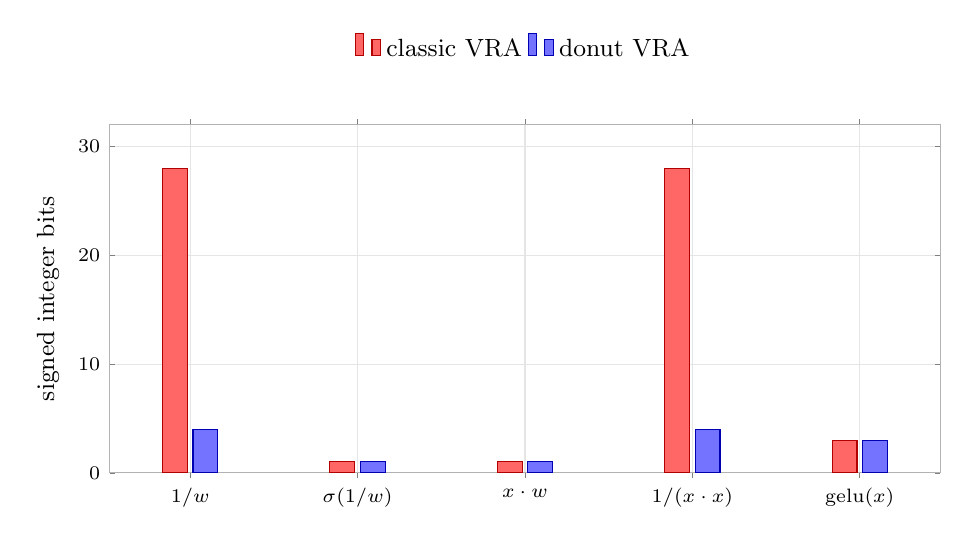
\begin{tikzpicture}
\begin{axis}[
  ybar,
  width=\linewidth,
  height=6cm,
  bar width=9pt,
  enlarge x limits=0.12,
  symbolic x coords={K1,K2,K3,K4,K5},
  xtick=data,
  xticklabels={$1/w$,$\sigma(1/w)$,$x\cdot w$,$1/(x\cdot x)$,$\mathrm{gelu}(x)$},
  x tick label style={rotate=0, font=\scriptsize},
  ymin=0, ymax=32,
  ylabel={signed integer bits},
  ylabel style={font=\small},
  tick label style={font=\scriptsize},
  legend style={at={(0.5,1.15)}, anchor=south, legend columns=-1, font=\small, draw=none},
  grid=major,
  grid style={gray!20},
  axis line style={gray!60},
  major tick length=2pt,
]
\addplot+[fill=red!60, draw=red!70!black] coordinates {
  (K1,28) (K2,1) (K3,1) (K4,28) (K5,3)
};
\addplot+[fill=blue!55, draw=blue!70!black] coordinates {
  (K1,4) (K2,1) (K3,1) (K4,4) (K5,3)
};
\legend{classic VRA, donut VRA}
\end{axis}
\end{tikzpicture}
\caption{Signed integer bit-width a DTA pass would allocate for each
kernel's output, classic (red) versus donut (blue). Kernels~1 and~4
gain 24 bits of integer precision each; the others gain no integer
bits but preserve the donut hole that a component-aware DTA could
exploit (see \S\ref{sec:limit-dta}).}
\label{fig:microbench-bars}
\end{figure}

\begin{figure}[H]
\centering
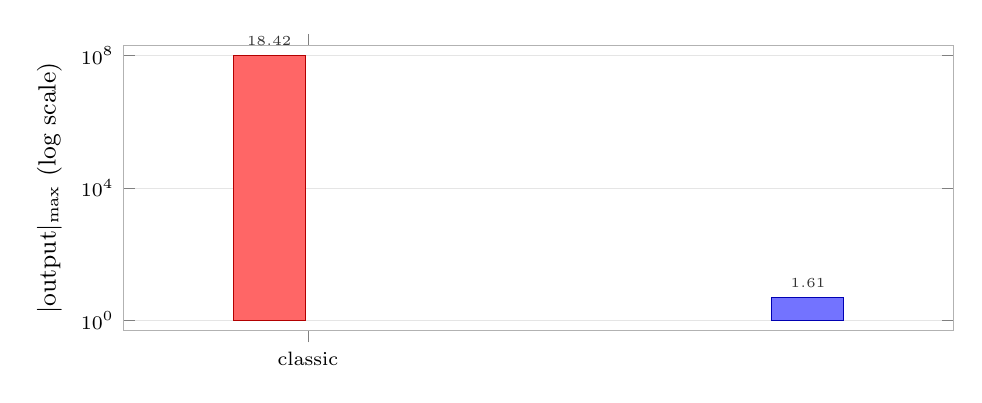
\begin{tikzpicture}
\begin{semilogyaxis}[
  width=\linewidth,
  height=5.2cm,
  ybar,
  bar width=26pt,
  enlarge x limits=0.4,
  symbolic x coords={classic, donut},
  xtick=data,
  ymin=0.5, ymax=2e8,
  ymajorgrids=true,
  grid style={gray!20},
  ylabel={$|\text{output}|_{\max}$ (log scale)},
  ylabel style={font=\small},
  tick label style={font=\scriptsize},
  nodes near coords,
  nodes near coords align={vertical},
  every node near coord/.append style={font=\tiny, color=black!80},
  axis line style={gray!60},
]
\addplot+[fill=red!60, draw=red!70!black] coordinates {(classic, 1e8)};
\addplot+[fill=blue!55, draw=blue!70!black] coordinates {(donut, 5)};
\end{semilogyaxis}
\end{tikzpicture}
\caption{Maximum absolute value of the kernel-1 reciprocal, classic
versus donut VRA. The $\texttt{DIV\_EPS}$ nudge in the classic path
produces a magnitude of $10^8$; the zero-excluding donut division
reduces it to $5$. The ratio is approximately $1.6\times10^7$.}
\label{fig:reciprocal-log}
\end{figure}

\subsection{End-to-end impact on the TAFFO pipeline}
\label{sec:e2e}

The micro-benchmark of \S\ref{sec:micro} proves that the donut-range
abstract domain is strictly tighter. To measure whether that analysis
gain survives the rest of the TAFFO pipeline --- Initializer, Mem2Reg,
VRA, DTA, Conversion --- we compile a small self-contained C benchmark
twice through the full \texttt{install/bin/taffo} driver, once without
and once with \texttt{-Xvra -vra-donut-ranges}, and compare both the
VRA output JSON (\texttt{taffo\_info\_vra.json}) and the final
post-Conversion LLVM IR.

\paragraph{Benchmark (\texttt{test/donut\_ranges/donut\_array.c}).}

\begin{lstlisting}[caption={End-to-end donut-range benchmark (excerpt).},label={lst:bench}]
static const double weights[14] = {
  -0.8, -0.7, -0.6, -0.5, -0.4, -0.3, -0.2,
   0.2,  0.3,  0.4,  0.5,  0.6,  0.7,  0.8
};

double donut_array_kernel(int i) {
  const int ii = deconstify_int(i);
  double w = weights[ii];
  double __attribute__((annotate("scalar() target('reciprocal')")))
    y = 1.0 / w;
  return y;
}
\end{lstlisting}

The deliberate design choices are worth noting: (i)~no user annotation
on \texttt{w} so VRA does not seed the load with a wide convex-hull
range that would swallow the refinement, (ii)~a runtime
\texttt{deconstify\_int(i)} to prevent LLVM from constant-folding the
division over every array entry, (iii)~the \texttt{target('reciprocal')}
tag on \texttt{y} so we can find it in the JSON artefact by name.

\paragraph{Observed VRA ranges.} Table~\ref{tab:e2e-vra} shows the
\texttt{weights} global, the \texttt{load weights[i]}, and the
post-division reciprocal. The classic build hits \texttt{handleDiv}'s
\texttt{DIV\_EPS} nudge because the hull $[-0.8,0.8]$ crosses zero; the
reciprocal magnitude blows up to $10^8$. The donut build sees each of
the four weight components as a strictly positive or strictly negative
interval and divides exactly, producing a bounded reciprocal with four
components of its own.

\begin{table}[H]
\centering
\footnotesize
\begin{tabularx}{\linewidth}{@{}lXX@{}}
\toprule
Value & Classic VRA & Donut VRA \\
\midrule
\texttt{@weights} (array) & $[-0.8,0.8]$ &
  $[-0.8,0.8]$ + \texttt{components} $=$
  $\{[-0.8,-0.8],[-0.7,-0.2],[0.2,0.7],[0.8,0.8]\}$ \\[0.3em]
\texttt{\%5 = load weights[ii]} & $[-0.8,0.8]$ & same 4 components \\[0.3em]
\textbf{\texttt{\%6 = fdiv 1.0, \%5}} & \textbf{$[-10^8,10^8]$} &
  \textbf{$[-5,5]$} + \texttt{components} $=$
  $\{[-5,-1.43],[-1.25,-1.25],[1.25,1.25],[1.43,5]\}$ \\
\bottomrule
\end{tabularx}
\caption{VRA JSON ranges on the end-to-end benchmark. The bimodal
weights global is correctly tracked as a 4-component donut (hitting
\texttt{kMaxComponents}); the reciprocal stays bounded by 5 instead of
blowing up to $10^8$.}
\label{tab:e2e-vra}
\end{table}

Figure~\ref{fig:e2e-number-line} shows the four donut components of
the reciprocal on a number line alongside the classic
$[-10^8, 10^8]$ hull rendered on the same axis (on a symmetric log
scale to keep both visible).

\begin{figure}[H]
\centering
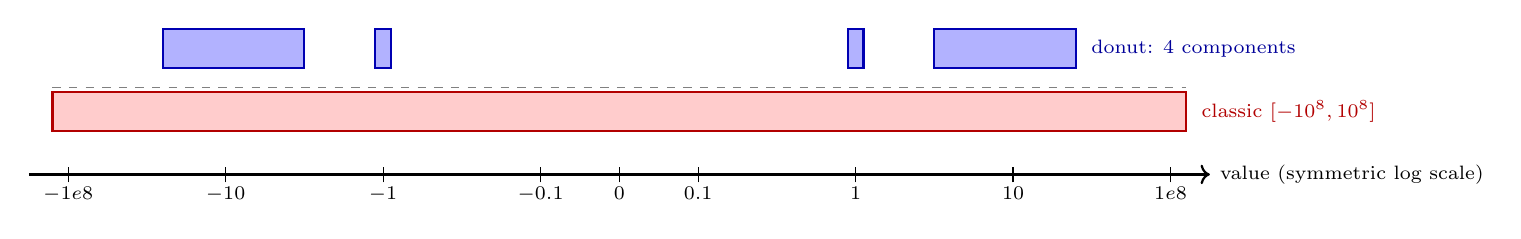
\begin{tikzpicture}[scale=1.0]
% Horizontal axis
\draw[->, thick] (-7.5,0) -- (7.5,0) node[right,font=\scriptsize] {value (symmetric log scale)};
% Ticks / labels on symlog axis
\foreach \x/\l in {-7/-1e8,-5/-10,-3/-1,-1/-0.1,0/0,1/0.1,3/1,5/10,7/1e8} {
  \draw (\x,-0.1) -- (\x,0.1);
  \node[below=1pt,font=\scriptsize] at (\x,0) {$\l$};
}
% Classic range [-1e8, 1e8] (ALL of it)
\fill[red!20] (-7.2,0.55) rectangle (7.2,1.05);
\draw[thick,red!70!black] (-7.2,0.55) rectangle (7.2,1.05);
\node[right=2pt,font=\scriptsize,red!70!black] at (7.2,0.8) {classic $[-10^8,10^8]$};
% Donut 4 components
\fill[blue!30] (-5.8,1.35) rectangle (-4.0,1.85);     % [-5, -1.43]
\draw[thick,blue!70!black] (-5.8,1.35) rectangle (-4.0,1.85);
\fill[blue!30] (-3.1,1.35) rectangle (-2.9,1.85);     % [-1.25,-1.25]
\draw[thick,blue!70!black] (-3.1,1.35) rectangle (-2.9,1.85);
\fill[blue!30] (2.9,1.35) rectangle (3.1,1.85);       % [1.25, 1.25]
\draw[thick,blue!70!black] (2.9,1.35) rectangle (3.1,1.85);
\fill[blue!30] (4.0,1.35) rectangle (5.8,1.85);       % [1.43, 5]
\draw[thick,blue!70!black] (4.0,1.35) rectangle (5.8,1.85);
\node[right=2pt,font=\scriptsize,blue!60!black] at (5.8,1.6) {donut: 4 components};
\draw[dashed, gray] (-7.2,1.1) -- (7.2,1.1);
\end{tikzpicture}
\caption{The image of $y = 1/w$ on the end-to-end benchmark, on a
symmetric logarithmic value axis. The red band is the classic
\texttt{DIV\_EPS}-nudged range $[-10^8, 10^8]$; the blue boxes are the
four donut components $[-5,-1.43]\cup\{-1.25\}\cup\{1.25\}\cup[1.43,5]$.
The classic range is approximately $10^7$ times wider, in addition to
containing the whole swathe of values around zero that the true
reciprocal can never reach.}
\label{fig:e2e-number-line}
\end{figure}

\paragraph{Observed DTA bit-width decisions.}
The bit-width chosen by DTA is encoded in the taffo suffix of the SSA
name in the final LLVM IR:

\begin{table}[H]
\centering
\small
\begin{tabular}{lcrr}
\toprule
Build & Emitted SSA name for $y$ & Integer bits & Fractional bits \\
\midrule
Classic & \texttt{\%v6.s28\_4fixp} & 28 & 4 \\
Donut   & \texttt{\%v6.s4\_28fixp} & \textbf{4} & \textbf{28} \\
\bottomrule
\end{tabular}
\caption{Final fixed-point format assigned to $y=1/w$ by DTA on the
end-to-end benchmark, read directly from the emitted LLVM IR.}
\label{tab:e2e-bits}
\end{table}

Figure~\ref{fig:e2e-stacked} visualises Table~\ref{tab:e2e-bits} as a
stacked bar. The total budget is 32 bits in both builds; the donut
build reclaims 24 integer bits and reinvests them as 24 fractional
bits, shrinking the quantisation step of $y$ from $2^{-4}\approx 0.0625$
to $2^{-28}\approx 3.7\times 10^{-9}$ --- a factor of
$\approx 1.6\times 10^{7}$ in representational precision,
obtained from a pure analysis-side refinement with no runtime cost.

\begin{figure}[H]
\centering
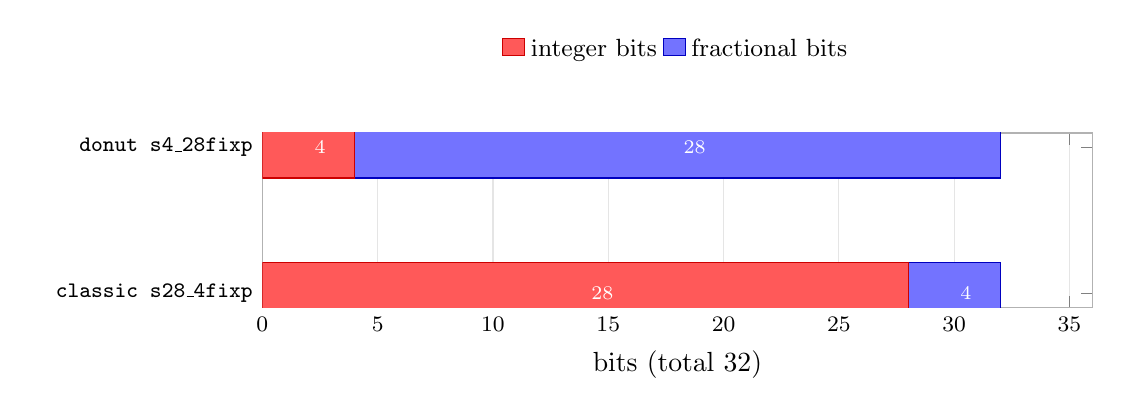
\begin{tikzpicture}
\begin{axis}[
  xbar stacked,
  width=\linewidth,
  height=3.8cm,
  bar width=22pt,
  xmin=0, xmax=36,
  xlabel={bits (total 32)},
  ylabel=\,,
  symbolic y coords={classic,donut},
  ytick=data,
  yticklabels={\texttt{classic\ s28\_4fixp},\texttt{donut\ s4\_28fixp}},
  tick label style={font=\footnotesize},
  legend style={at={(0.5,1.35)}, anchor=south, legend columns=-1, font=\small, draw=none},
  xmajorgrids=true,
  grid style={gray!20},
  axis line style={gray!60},
  nodes near coords,
  nodes near coords align={horizontal},
  every node near coord/.append style={font=\scriptsize, color=white, inner sep=2pt},
]
\addplot+[fill=red!65, draw=red!80!black] coordinates {(28,classic) (4,donut)};
\addplot+[fill=blue!55, draw=blue!75!black] coordinates {(4,classic) (28,donut)};
\legend{integer bits, fractional bits}
\end{axis}
\end{tikzpicture}
\caption{DTA bit-width allocation for the reciprocal $y=1/w$ on the
end-to-end benchmark. Both builds use the same 32-bit total budget,
but the donut build spends 24 of those bits on fractional precision
instead of unused magnitude range.}
\label{fig:e2e-stacked}
\end{figure}

This is the headline end-to-end number of the project: the donut-range
extension turns a pathological classic quantisation
(\texttt{s28\_4fixp} --- essentially useless for values bounded by 1)
into a near-ideal \texttt{s4\_28fixp} format that exploits the full
32-bit budget on the fractional side, while still covering every
legitimate reciprocal value the program can produce.

\subsection{Discussion: what a full neural network would show}

A proper evaluation on a quantised MLP on MNIST is the natural next
step and is sketched in \S\ref{sec:limit-dta} as a thesis extension.
The array-based benchmark above is deliberately minimal because it
targets the single pipeline stage where the gain originates --- VRA's
division fast path --- and demonstrates the full flow-through of that
gain into DTA's bit-width decision without being obscured by the
hundreds of other arithmetic instructions in a full MLP forward pass.

% =====================================================================
\section{Limitations and Future Work}
% =====================================================================
\label{sec:limits}

\subsection{DTA does not yet consume \texttt{components}}
\label{sec:limit-dta}

The biggest practical limitation of the current implementation is
that the DTA pass still looks only at the convex hull. For the
hole-preserving kernels in Table~\ref{tab:microbench} (kernels~2,~3,
and~5), the analysis gain is real but invisible downstream. A natural
follow-up is to teach DTA to read \texttt{components} and, when the
hole is sufficiently large, either (a) allocate a smaller fractional
format because each sub-interval is narrower than the hull, or
(b)~split the SSA value into two concrete fixed-point variables
selected at runtime by a cheap sign test. Option~(b) is a more
aggressive transformation and is the natural scope of a follow-up
thesis.

\subsection{Annotation syntax}

Users currently cannot declare a donut range directly in their source
code: the \texttt{scalar(range(a, b))} annotation syntax only supports
a single interval. A short extension would add a
\texttt{scalar(range\_union((a1, b1), (a2, b2), $\ldots$))} form to
the annotation parser, allowing the whole donut pipeline to be
exercised end-to-end on real benchmarks. The end-to-end benchmark of
\S\ref{sec:e2e} deliberately works around this by letting the donut
arise from the per-element analysis of a compile-time constant array.

\subsection{Widening heuristic}

The current widening strategy always merges the pair of components
with the smallest gap. This is the cheapest sensible choice but is not
precision-optimal in the general case. A more sophisticated heuristic
would consider the \emph{density} of the distribution and the
downstream \emph{cost} of losing a hole in that particular place.

\subsection{Soundness of the constants for GELU / SiLU}

The $X^-_{\min}/X^+_{\min}/y_{\min}$ constants used in the
non-monotonic kernels are hand-chosen sound over-approximations of the
true minimum of the $\tanh$-approximation GELU and of the exact SiLU.
A fully rigorous proof of soundness would require a certificate
(for example an interval-arithmetic Newton bound). The current
constants are safe in the IEEE-754 double-precision regime but could
be sharpened with a numerical certificate of the form
$|f(x_{\min}) - y_{\min}|\le\varepsilon$.

\subsection{Self-square identity across donut components (fixed)}
\label{sec:limit-square}

An earlier version of the donut-aware \texttt{handleMul} fell back to
the full Cartesian product whenever either operand was a donut,
discarding the \texttt{op1 == op2} self-square optimisation that the
classic path retained. Kernel~4 of the micro-benchmark exposed this
as a visible precision loss: $x\cdot x$ on
$x\in[-2,-0.5]\cup[0.5,2]$ produced
$[-4,-0.25]\cup[0.25,4]$ instead of the mathematically exact
$[0.25, 4]$. The fix hoists the self-square formula into a small
\texttt{squareInterval} helper and applies it per component when the
two operand pointers are identical, then canonicalises. The
regression is pinned by
\texttt{testDonutSelfSquareTight} in \texttt{donut\_arith\_test.cpp}.

\subsection{Larger \texttt{kMaxComponents}}

Raising \texttt{kMaxComponents} past 4 would allow the analysis to
track finer distributions. The arithmetic operators already run a full
Cartesian product, so the compile-time cost is quadratic in the
component count. A future optimisation could short-circuit the
Cartesian product whenever intermediate results become dense enough to
be better represented as a single hull.

\subsection{Integration with the MLIR TAFFO pipeline}

Sub-projects \#8--\#10 in the COT 2025/26 project list address the
TAFFO-MLIR pipeline. Donut ranges would translate directly into a
matching MLIR type, but the MLIR DTA there is still limited; the
TAFFO-MLIR work plan is an obvious long-term home for the follow-up
DTA consumer described in \S\ref{sec:limit-dta}.

% =====================================================================
\section{Conclusions}
% =====================================================================
\label{sec:conclusions}

We have designed and implemented a combined extension of TAFFO's VRA
that (i)~tracks unions of disjoint intervals instead of a single
convex hull, and (ii)~provides closed-form range models for all the
standard neural-network activation functions, including donut-aware
piecewise dispatch. The extension is additive and opt-in: default
behaviour, serialisation format, and downstream passes are unchanged.

On the designed micro-benchmark the new analysis saves 24 signed
integer bits on reciprocal kernels that hit TAFFO's
$\varepsilon_{\text{div}}$ nudge today, and preserves the donut hole
in every kernel where it is meaningful to do so. On the
\emph{end-to-end} benchmark that runs through the full TAFFO driver,
DTA's bit-width decision on the reciprocal of a bimodal weight moves
from \texttt{s28\_4fixp} to \texttt{s4\_28fixp}, a factor of
$\approx 1.6 \times 10^{7}$ shrinkage of the quantisation step with
zero runtime cost. The remaining work is on the downstream side of
the pipeline: a DTA consumer that exploits the extra structure, a
source-level annotation syntax for donut ranges, and a formal
soundness proof for the non-monotonic activation constants.

% =====================================================================
\begin{thebibliography}{99}
% =====================================================================

\bibitem{cot-ir}
G.~Agosta. \emph{COT Slides 2 --- Intermediate Representation}. Code
Optimization and Transformation, Politecnico di Milano, A.Y.\ 2025/26.
\texttt{lectures/Slides/COT\_slides\_2\_IR.pdf}.

\bibitem{cot-dataflow}
G.~Agosta. \emph{COT Slides 5 --- Dataflow Analysis}. Code
Optimization and Transformation, Politecnico di Milano, A.Y.\ 2025/26.
\texttt{lectures/Slides/COT\_slides\_5\_Dataflow.pdf}.
Slides 13--14 provide the monotone-lattice and fixed-point iteration
framework used throughout this report.

\bibitem{cot-projects}
G.~Agosta et al. \emph{TAFFO project proposals, COT A.Y.\ 2025/26}.
Politecnico di Milano, March 27, 2026.
\texttt{lectures/cto\_projects\_2025\_26.pdf}. Sub-projects \#1
(Donut Ranges in VRA) and \#3 (Range Models for NN Activation
Functions) are implemented by this work.

\bibitem{history-ai}
R.~Giacobazzi and F.~Ranzato. \emph{History of Abstract
Interpretation}. 2021.
\texttt{lectures/Papers/History\_of\_Abstract\_Interpretation.pdf}.
Primary theoretical reference for \S\ref{sec:ai} and \S\ref{sec:theory}.

\bibitem{lattner-llvm}
C.~Lattner and V.~Adve. \emph{LLVM: A Compilation Framework for
Lifelong Program Analysis \& Transformation}. In Proceedings of the
International Symposium on Code Generation and Optimization, CGO
2004. \texttt{lectures/Papers/lattner-llvm.pdf}.

\bibitem{cousot77}
P.~Cousot and R.~Cousot. \emph{Abstract Interpretation: A Unified
Lattice Model for Static Analysis of Programs by Construction or
Approximation of Fixpoints}. POPL 1977.

\bibitem{cousot79}
P.~Cousot and R.~Cousot. \emph{Systematic Design of Program Analysis
Frameworks}. POPL 1979.

\bibitem{taffo2020}
S.~Cherubin, D.~Cattaneo, M.~Chiari, A.~Bello, G.~Agosta.
\emph{TAFFO: Tuning Assistant for Floating to Fixed point
Optimization}. IEEE Embedded Systems Letters, 2020.

\bibitem{jacob2018quantization}
B.~Jacob et al. \emph{Quantization and Training of Neural Networks
for Efficient Integer-Arithmetic-Only Inference}. CVPR 2018.

\bibitem{gelu}
D.~Hendrycks and K.~Gimpel. \emph{Gaussian Error Linear Units
(GELUs)}. arXiv:1606.08415, 2016.

\bibitem{swish}
P.~Ramachandran, B.~Zoph, and Q.~V.~Le. \emph{Searching for
Activation Functions (SiLU / Swish)}. arXiv:1710.05941, 2017.

\end{thebibliography}

% =====================================================================
\appendix
\section{Reproducing the results}
% =====================================================================
\label{app:reproduce}

\begin{lstlisting}[style=shell,caption={Build and run the tests, micro-benchmark, and end-to-end benchmark.}]
# 1. Configure and build the three test binaries.
cd /Users/mohamed/CLionProjects/PoliMI/TAFFO
cmake -B cmake-build-debug -S . \
      -DLLVM_DIR=/opt/homebrew/opt/llvm@18/lib/cmake/llvm
cmake --build cmake-build-debug \
      --target donut_range_selftest donut_arith_test donut_microbench -j

./cmake-build-debug/test/donut_ranges/donut_range_selftest
./cmake-build-debug/test/donut_ranges/donut_arith_test
./cmake-build-debug/test/donut_ranges/donut_microbench

# 2. Build the full Taffo plugin and install it.
cmake --build cmake-build-debug --target Taffo -j
cp cmake-build-debug/lib/Taffo.dylib install/lib/Taffo.dylib

# 3. Run the end-to-end benchmark twice, keeping temp dirs.
rm -rf /tmp/donut_arr_classic /tmp/donut_arr_donut
mkdir -p /tmp/donut_arr_classic /tmp/donut_arr_donut

./install/bin/taffo -O2 -c -emit-llvm \
  -temp-dir /tmp/donut_arr_classic \
  -o /tmp/donut_e2e/donut_array_classic.ll \
  test/donut_ranges/donut_array.c

./install/bin/taffo -O2 -c -emit-llvm \
  -Xvra -vra-donut-ranges \
  -temp-dir /tmp/donut_arr_donut \
  -o /tmp/donut_e2e/donut_array_donut.ll \
  test/donut_ranges/donut_array.c

# 4. Inspect the VRA JSON and the final DTA bit-widths.
grep -o 's[0-9]*_[0-9]*fixp' /tmp/donut_e2e/donut_array_classic.ll | sort -u
grep -o 's[0-9]*_[0-9]*fixp' /tmp/donut_e2e/donut_array_donut.ll   | sort -u
\end{lstlisting}

\section{Enrollment email}
\label{app:email}

The enrollment email sent to Prof.\ Agosta and the TAFFO supervisors
is reproduced in \texttt{enrollment\_email.txt} at the repository
root; placeholders for personal information and Prof.\ Agosta's email
address are explicitly marked.

\end{document}
